\documentclass{beamer}

\usepackage{graphicx}
\usepackage{listings}
\usetheme{Szeged}
\usecolortheme{beaver}

\author{Anne Wanningen \and Xeryus Stokkel}
\title[Week 4]{Introduction to Computer Graphics OpenGL week 4}

\begin{document}

\maketitle

\section{Results}
\begin{frame}
	\begin{figure}
		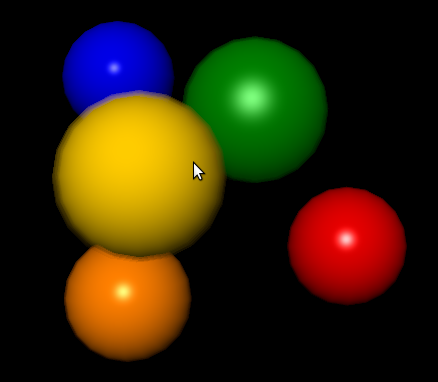
\includegraphics[height=.90\textheight]{result.png}
	\end{figure}
\end{frame}

\section{Depth of Field}
\begin{frame}
	\begin{columns}[T]
		\begin{column}{.5\textwidth}
			\begin{figure}
				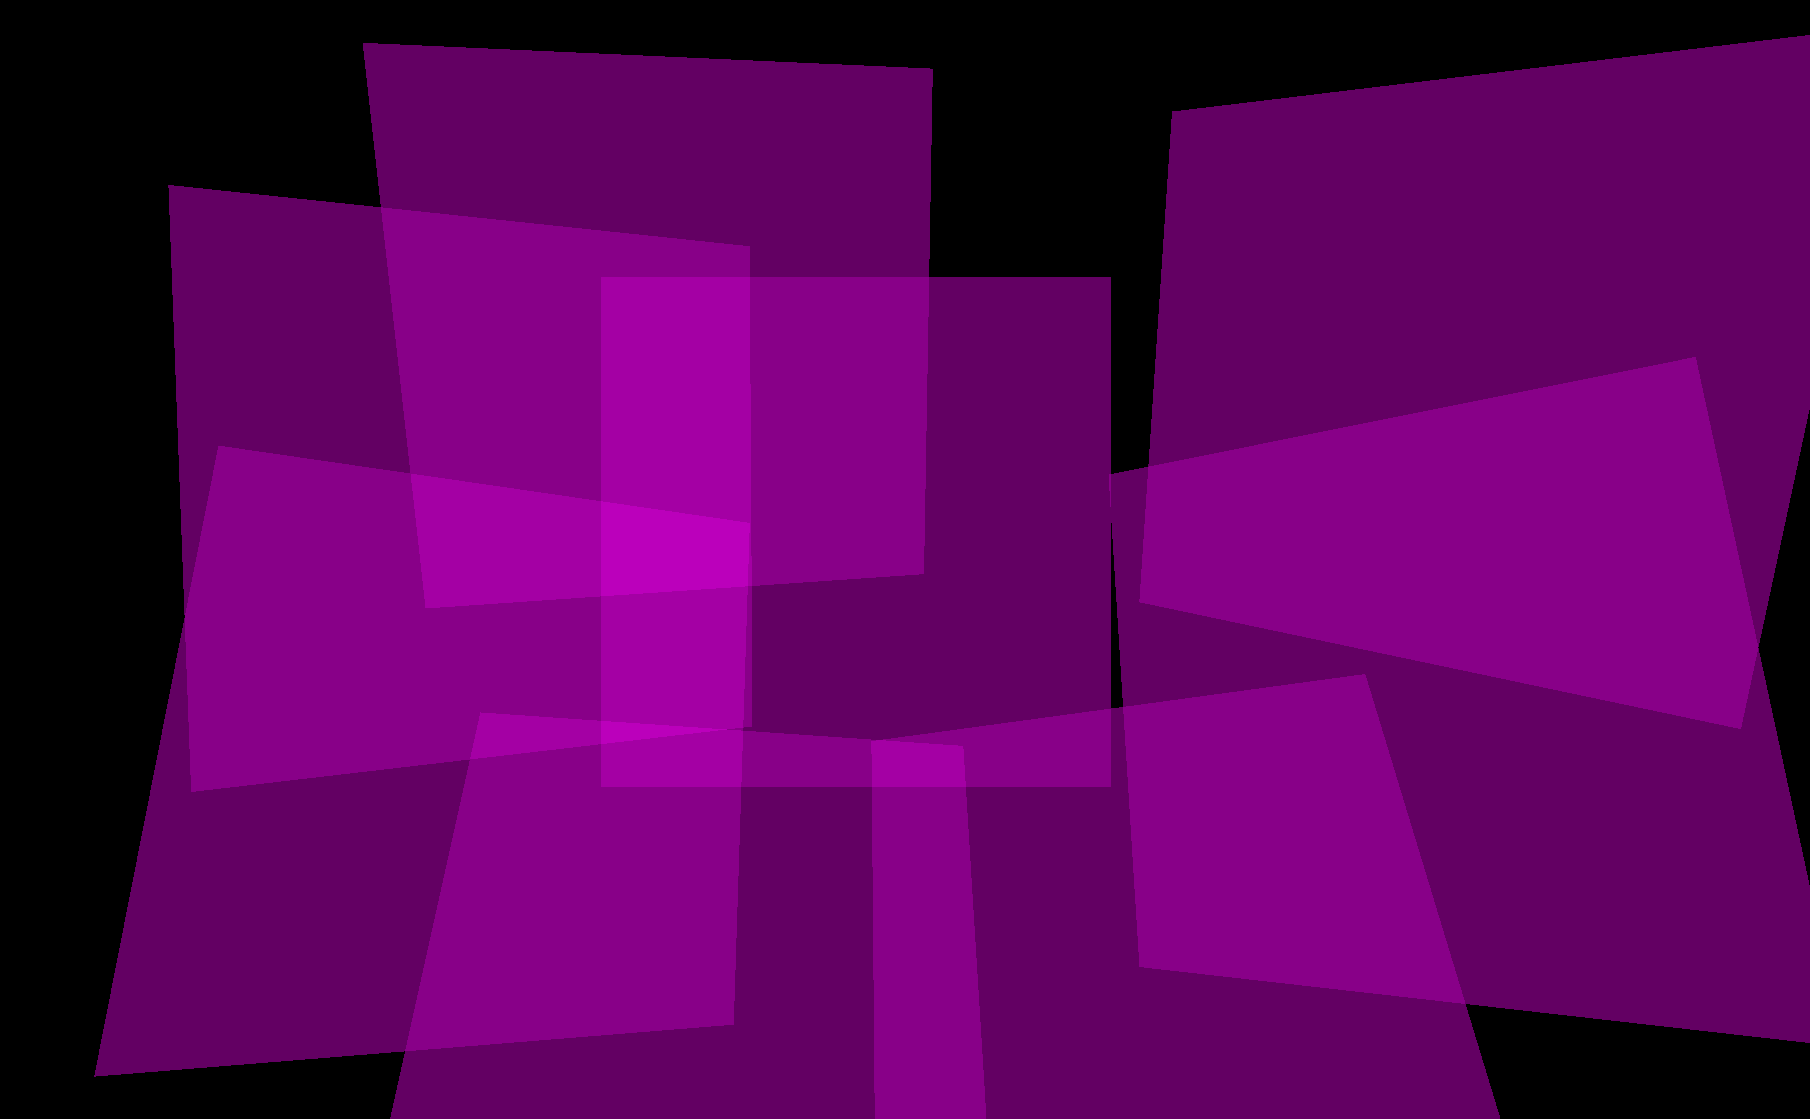
\includegraphics[width=\textwidth]{blurryCubes.png}
			\end{figure}
		\end{column}
		\begin{column}{.5\textwidth}
			\begin{figure}
				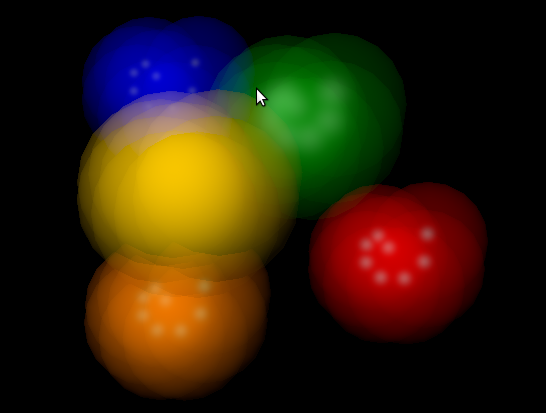
\includegraphics[width=\textwidth]{blurryBalls.png}
			\end{figure}
		\end{column}
	\end{columns}
\end{frame}

\section{Meshes}
\begin{frame}
	\begin{columns}[T]
		\begin{column}{.45\textwidth}
			Loads of black screens with little indication of the cause.
		\end{column}
		\begin{column}{.45\textwidth}
			\begin{figure}
				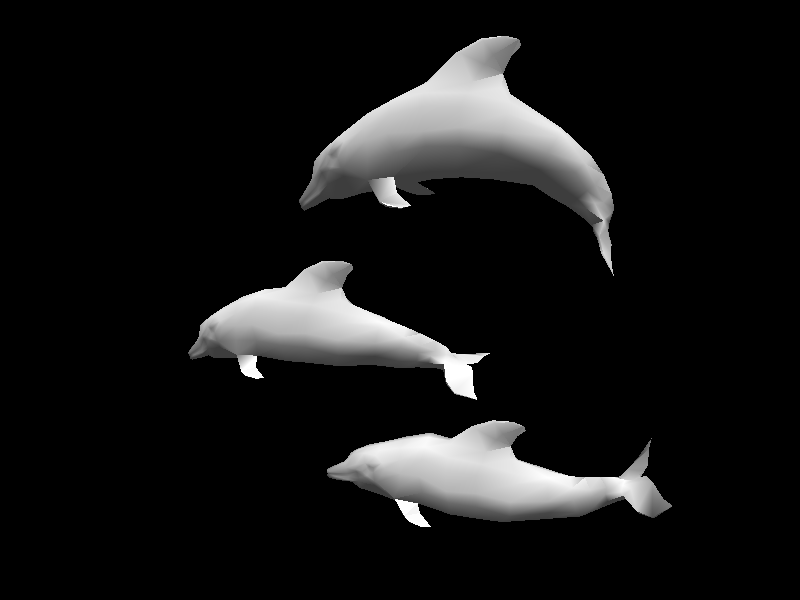
\includegraphics[width=\textwidth]{dolphins.png}
			\end{figure}
		\end{column}
	\end{columns}
\end{frame}

\begin{frame}
	\begin{columns}[T]
		\begin{column}{.45\textwidth}
			\begin{figure}
				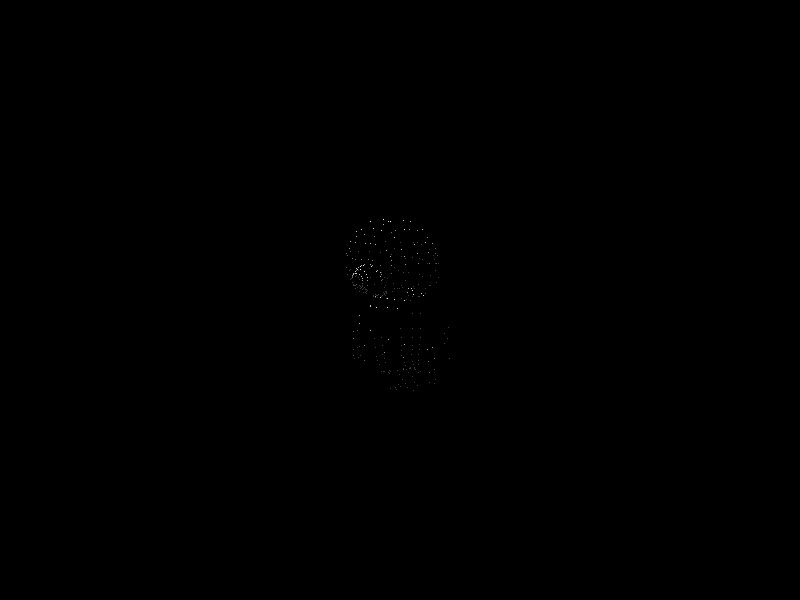
\includegraphics[width=\textwidth]{teddy.png}
			\end{figure}
		\end{column}
	\end{columns}
\end{frame}

\begin{frame}[fragile]
	Vertex/normal pair deduplication: barely useful, sometimes leads to blank screens, quite slow.
	\begin{lstlisting}
	$ ./openglframework -m obj/cube.obj -r
	Triangle count:    12
	Normal count:      32
	Expected vertices: 36
	Actual vertices:   32
	Stored indices:    36
	\end{lstlisting}
\end{frame}

\begin{frame}[fragile]
	\begin{lstlisting}
	$ ./openglframework -m obj/devilduk.obj -r
	Triangle count:    3712
	Normal count:      1976
	Expected vertices: 11136
	Actual vertices:   11136
	Stored indices:    11136
	\end{lstlisting}
	\begin{lstlisting}
	$ ./openglframework -m obj/dolphins.obj -r
	Triangle count:    1692
	Normal count:      1202
	Expected vertices: 5076
	Actual vertices:   5076
	Stored indices:    5076
	\end{lstlisting}
\end{frame}

\end{document}
